\documentclass[tikz,border=3pt]{standalone}
\usepackage{newtxtext,newtxmath}
\usetikzlibrary{arrows.meta}
\definecolor{paperink}{HTML}{3F4852}
\definecolor{paperblue}{HTML}{2457C5}
\definecolor{paperred}{HTML}{C43B3B}
\definecolor{papergreen}{HTML}{2E8B57}
\definecolor{papergray}{HTML}{F1F3F5}
\begin{document}
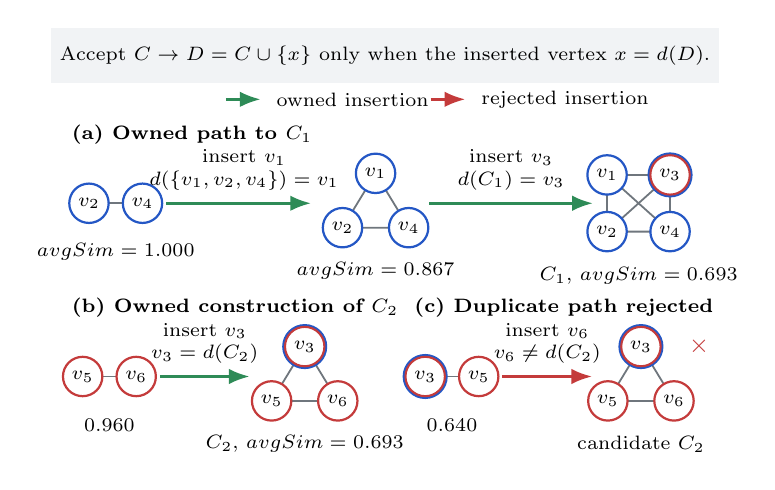
\begin{tikzpicture}[
  font=\scriptsize,
  >=Latex,
  vertex/.style={circle, draw=paperblue, fill=white, line width=0.8pt,
    minimum size=5.0mm, inner sep=0pt, font=\scriptsize},
  mone/.style={vertex, draw=paperblue},
  mtwo/.style={vertex, draw=paperred},
  vthree/.style={vertex, draw=paperred, line width=0.75pt,
    preaction={draw=paperblue, line width=2.05pt}},
  edge/.style={draw=paperink!75, line width=0.65pt},
  owned/.style={->, draw=papergreen, line width=1.0pt},
  duplicate/.style={->, draw=paperred, line width=1.0pt},
  paneltitle/.style={font=\scriptsize\bfseries, anchor=west},
  note/.style={font=\scriptsize, align=center},
  rule/.style={draw=none, fill=papergray,
    minimum width=84mm, minimum height=7mm, align=center}
]

% Canonical rule shared by all panels.
\node[rule] at (4.20,1.18)
  {Accept $C\rightarrow D=C\cup\{x\}$ only when the inserted vertex $x=d(D)$.};
\draw[owned] (2.18,0.62)--(2.62,0.62);
\node[anchor=west, font=\scriptsize] at (2.70,0.62) {owned insertion};
\draw[duplicate] (4.78,0.62)--(5.22,0.62);
\node[anchor=west, font=\scriptsize] at (5.30,0.62) {rejected insertion};

% Panel (a): the owned path to C1.
\node[paneltitle] at (0.10,0.17) {(a) Owned path to $C_1$};

\begin{scope}[shift={(0.78,-0.70)}]
  \draw[edge] (-0.34,0)--(0.34,0);
  \node[mone] at (-0.34,0) {$v_2$};
  \node[mone] at ( 0.34,0) {$v_4$};
  \node[note] at (0,-0.62) {$\operatorname{avgSim}=1.000$};
\end{scope}

\begin{scope}[shift={(4.08,-0.70)}]
  \draw[edge] (0,0.38)--(-0.42,-0.31)--(0.42,-0.31)--cycle;
  \node[mone] at (0,0.38) {$v_1$};
  \node[mone] at (-0.42,-0.31) {$v_2$};
  \node[mone] at ( 0.42,-0.31) {$v_4$};
  \node[note] at (0,-0.86) {$\operatorname{avgSim}=0.867$};
\end{scope}

\begin{scope}[shift={(7.42,-0.70)}]
  \coordinate (a) at (-0.40, 0.36);
  \coordinate (b) at (-0.40,-0.36);
  \coordinate (c) at ( 0.40, 0.36);
  \coordinate (d) at ( 0.40,-0.36);
  \draw[edge] (a)--(b)--(d)--(c)--cycle (a)--(d) (b)--(c);
  \node[mone] at (a) {$v_1$};
  \node[mone] at (b) {$v_2$};
  \node[vthree] at (c) {$v_3$};
  \node[mone] at (d) {$v_4$};
  \node[note] at (0,-0.92) {$C_1$, $\operatorname{avgSim}=0.693$};
\end{scope}

\draw[owned] (1.42,-0.70)--(3.26,-0.70)
  node[midway,above=0.35mm,note,xshift=0.7mm] {insert $v_1$\\$d(\{v_1,v_2,v_4\})=v_1$};
\draw[owned] (4.76,-0.70)--(6.84,-0.70)
  node[midway,above=0.35mm,note] {insert $v_3$\\$d(C_1)=v_3$};

% Panel (b): accepted construction of C2.
\node[paneltitle] at (0.10,-2.03) {(b) Owned construction of $C_2$};
\begin{scope}[shift={(0.70,-2.90)}]
  \draw[edge] (-0.34,0)--(0.34,0);
  \node[mtwo] at (-0.34,0) {$v_5$};
  \node[mtwo] at ( 0.34,0) {$v_6$};
  \node[note] at (0,-0.62) {$0.960$};
\end{scope}
\begin{scope}[shift={(3.18,-2.90)}]
  \draw[edge] (0,0.38)--(-0.42,-0.31)--(0.42,-0.31)--cycle;
  \node[vthree] at (0,0.38) {$v_3$};
  \node[mtwo] at (-0.42,-0.31) {$v_5$};
  \node[mtwo] at ( 0.42,-0.31) {$v_6$};
  \node[note] at (0,-0.86) {$C_2$, $\operatorname{avgSim}=0.693$};
\end{scope}
\draw[owned] (1.34,-2.90)--(2.48,-2.90)
  node[midway,above=0.35mm,note] {insert $v_3$\\$v_3=d(C_2)$};

% Panel (c): alternative insertion creates C2 but is not owned.
\node[paneltitle] at (4.45,-2.03) {(c) Duplicate path rejected};
\begin{scope}[shift={(5.05,-2.90)}]
  \draw[edge] (-0.34,0)--(0.34,0);
  \node[vthree] at (-0.34,0) {$v_3$};
  \node[mtwo] at ( 0.34,0) {$v_5$};
  \node[note] at (0,-0.62) {$0.640$};
\end{scope}
\begin{scope}[shift={(7.45,-2.90)}]
  \draw[edge] (0,0.38)--(-0.42,-0.31)--(0.42,-0.31)--cycle;
  \node[vthree] at (0,0.38) {$v_3$};
  \node[mtwo] at (-0.42,-0.31) {$v_5$};
  \node[mtwo] at ( 0.42,-0.31) {$v_6$};
  \node[font=\small\bfseries, text=paperred] at (0.74,0.39) {$\times$};
  \node[note] at (0,-0.86) {candidate $C_2$};
\end{scope}
\draw[duplicate] (5.69,-2.90)--(6.83,-2.90)
  node[midway,above=0.35mm,note] {insert $v_6$\\$v_6\neq d(C_2)$};

\end{tikzpicture}
\end{document}
